\section{Grundlagen}

\subsection{Warum Identity Management}
\frame{\frametitle{Warum Identity Management}

\begin{center}
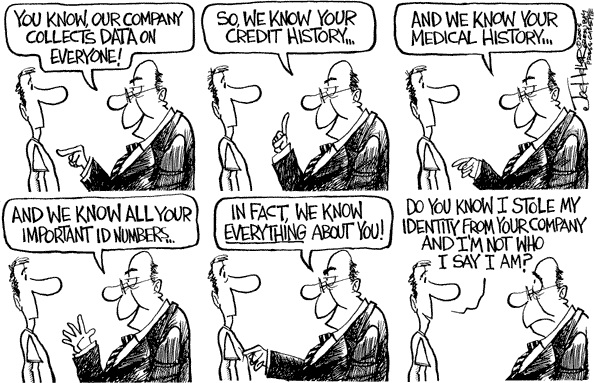
\includegraphics[scale=0.6]{pic/heller}
\end{center}

}

\frame{\frametitle{Warum Identity Management}

\begin{itemize}
\item Komplexer und wichtiger werdende IT Systeme
\item Steigende (digitale) Wirtschaftsspionage
\item Gesetzliche Anforderungen an den Datenschutz
\item Zeitdruck durch globale Wirtschaft und Konkurrenz
\end{itemize}

}

\subsection{Definitionen}

\subsubsection{Identität}
\frame{\frametitle{Identität}

\begin{shadequote}
Identität ist die Summe derjenigen Merkmale, anhand derer ein Individuum von anderen unterschieden werden kann.
\end{shadequote}

Wir beschränken wir uns auf die Merkmale welche digital erfassbar sind. Dazu zählen
ebenfalls gängige biometrische Verfahren.
}

\subsubsection{User}
\frame{\frametitle{User}
Hierbei handelt es sich in erster Linie um einen Menschen, welcher zum Sinne seiner Aufgabenerfüllung ein IT System nutzt. Es kann sich auch um einen \emph{virtuellen User} handeln. Dies ist der Fall wenn ein Programm über Rechte verfügt über welche es auf Ressourcen im Netzwerk zugreifen kann.
}

\subsubsection{Identity Management}
\frame{\frametitle{Identity Management}
Ist die Summe aller Maßnahmen, welche notwendig sind um einen User, eines IT Systems, eindeutig zu erkennen und ihn mit den entsprechenden Rechten zu versorgen, damit er seine Aufgaben ausführen kann. Alle diese Maßnahmen werden über standardisierte, nachvollziehbare Prozesse geregelt.
}

\subsubsection{Komplexität \& Zeit}
\frame{\frametitle{Komplexität \& Zeit}
Hierbei handelt es sich um die wichtigsten Faktoren welche das Identity Management beeinflussen. Die Komplexität bildet das benutzte IT System und das Betriebsorganigramm ab. Der Grad der Komplexität ist schon bei KMU recht hoch und wächst scheinbar exponentiell mit der Betriebsgröße. Zeit ist ein weiterer nicht zu unterschätzender Faktor, diese muss von zwei Seiten betrachtet werden. Zum einen muss das Identity Management in der Lage sein schnell auf eventuelle Änderungen bei den Usern zu reagieren. Zum anderen darf natürlich die Überprüfung der User Identität nicht zu viel seiner produktiven Zeit in Anspruch nehmen.
}